\documentclass[TFG.tex]{subfiles}

\begin{document}


%\hyphenation{equi-va-len-cia}\hyphenation{pro-pie-dad}\hyphenation{res-pec-ti-va-men-te}\hyphenation{sub-es-pa-cio}
\chapter{Peinado de trenzas}


En este capítulo veremos un algoritmo para resolver el problema de la palabra basado en la posibilidad de expresar las trenzas puras como elementos de un producto semidirecto de grupos libres. El algoritmo requerirá una técnica denominada \emph{peinado de trenzas} para que el orden de los factores sea el adecuado.

\section{Sucesiones exactas}
Hay dos sucesiones exactas relacionadas con los grupos de trenzas bien conocidas. La primera es bastante simple: a cada trenza de $B_n$ se le puede asociar la permutación que induce en sus cuerdas, esto es, un elemento del grupo simétrico $\Sigma_n$. Esto da lugar a un homomorfismo de grupos bien definido $\eta: B_n\to \Sigma_n$. Nótese que $\eta(\sigma_i)=(i\ i+1)$ para cada $i=1,\dots, n-1$. El núcleo de $\eta$ es el subgrupo de $B_n$ formado por las trenzas que inducen la permutación trivial, esto es, el grupo de trenzas puras $PB_n$. Por tanto, tenemos una sucesión exacta:
\begin{equation}\label{extension}
1\to PB_n\to B_n\overset{\eta}{\to}\Sigma_n\to 1.
\end{equation}

Hay también una aplicación que relaciona las trenzas puras de distintos índices. Concretamente, dada una trenza pura $\beta\in PB_{n+1}$, se puede eliminar, por ejemplo, la última cuerda para obtener una trenza pura $\rho(\beta)\in PB_n$. Esto da lugar a un homomorfismo de grupos bien definido $\rho: PB_{n+1}\to PB_n$, que es claramente sobreyectivo. El núcleo de esta aplicación consiste en las trenzas puras de $PB_{n+1}$ cuyas $n$ primeras cuerdas forman la trenza trivial. Salvo isotopía, podemos considerar que estas $n$ primeras cuerdas están en posición vertical. Si miramos este tipo de elementos como lazos en el espacio de configuración $M_{n+1}$, se corresponden al movimiento del $(n+1)$-ésimo punto mientras el resto de puntos permanecen quietos. Esto es por supuesto equivalente al movimiento de un punto en el plano complejo agujereado $n$ veces $\C_n$. En otras palabras, $\ker(\rho)=\pi_1(\C_n)\cong F_n$, por lo que tenemos la sucesión exacta:
\begin{equation}\label{pure}
1\to F_n \to PB_{n+1}\overset{\rho}{\to} PB_n\to 1.
\end{equation} 
En esta sucesión exacta, si $F_n$ está generado por $x_1,\dots, x_n$, vamos a ver que podemos definir $\iota: F_n\to PB_{n+1}$
\begin{gather*}
\iota(x_i)=A_{i,n+1},
\end{gather*}
donde $A_{i,n+1}$ son generadores de Birman (\ref{birman}). La aplicación está bien definida, es decir, la trenza resultante es pura por definición de los $A_{i,n+1}$. Para que sea la aplicación correcta y la sucesión sea exacta, $\iota$ debe ser inyectiva, que es lo siguiente que vamos a probar.
\begin{prop}\label{split}
La aplicación $\iota$ anteriormente definida es inyectiva.
\end{prop}
\begin{dem}
La idea de esta demostración será interpretar la sucesión exacta \ref{pure} en términos de otra que sabemos que es exacta y comprobar que $\iota$ es la aplicación correspondiente con esa otra interpretación.

Para $n\geq 1$ consideramos la aplicación
\begin{align}\label{fibrado}
p: & \qquad M_{n+1}\ \quad \longrightarrow\quad M_n\\
&(z_1,\dots,z_{n+1})\mapsto (z_1,\dots,z_n).\nonumber
\end{align} 

Nótese que que cada fibra $p^{-1}((z_1,\dots, z_n))$ es homeomorfa a $\C\setminus\{z_1,\dots, z_n\}=\C_n$. Como este espacio retrae con deformación sobre $S^1\lor\dots\lor S^1$, su grupo fundamental es $F_n$. De la sucesión exacta larga de grupos de homotopía asociada a $p$ de este fibrado \cite{Hatcher} obtenemos:
$$\pi_2(\C_n)\to\pi_2(M_{n+1})\to\pi_2(M_n)\to\pi_1(\C_n)\to\pi_1(M_{n+1})\to\pi_1(M_n)\to 1.$$
Se sabe que $\pi_2(\C_n)=1$ \cite{Hatcher}. Por otra parte, $\pi_2(M_1)=\pi_2(\C)={1}$. En la sucesión exacta anterior, esto implica que $\pi_2(M_2)=1$. Inductivamente se prueba que $\pi_2(M_n)=1$ para todo $n$. Esto da lugar a la sucesión exacta
$$1\to\pi_1(\C_n)\to\pi_1(M_{n+1})\to\pi_1(M_n)\to 1,$$
que por definición es equivalente a \ref{pure}. 


\begin{figure}[h!]
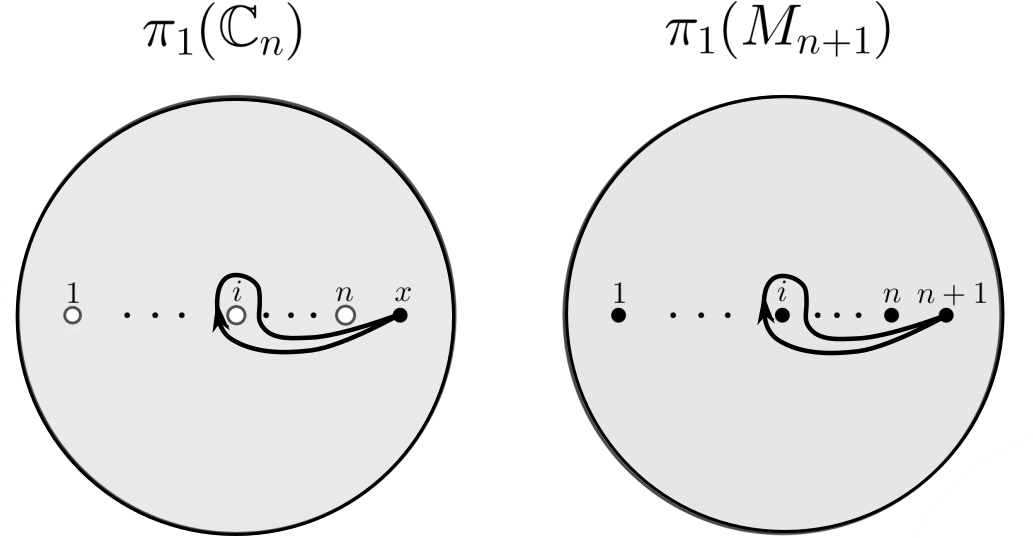
\includegraphics[scale=0.4]{Imagenes/inclusion.png}
\caption{Inclusión de $F_n$ en $PB_{n+1}$.}\label{inclusion}
\end{figure}\
%la fibra es homeomorfa a eso porque hay n puntos donde no podemos colocar el n+1
%\newpage
Si denotamos $j:\pi_1(\C_n)\to\pi_1(M_{n+1})$ a la aplicación natural de la anterior sucesión exacta, basta ver que $j$ coincide con $\iota$ para probar el resultado. Fijemos un punto base $x$ en $\C_n$ (véase la Figura \ref{inclusion}).

Como se puede comprobar, un lazo basado en $x$ en torno al agujero $i$-ésimo, que se corresponde con el generador $x_i$ de $F_n$, se transforma de modo natural en el movimiento del punto $n+1$ tal como se describe en la figura. Este movimiento es el que se corresponde con la trenza $A_{i,n+1}$, por lo que esta transformación es justamente la aplicación $\iota$. $\QED$
\end{dem}

%para ver que es homomorfismo basta notar que como es pura, el último hilo acaba siempre en el último punto, luego da igual quitarlo antes o después

%para ver que la sucesión es exacta basta que i sea inyectivo porque la imagen entonces será isomorfa a Fn


\newpage

\section{Trenzas puras como producto semidirecto de grupos libres}


Un hecho importante sobre la sucesión exacta \ref{pure} es que escinde. Para verlo, consideremos la aplicación $s:M_n\to M_{n+1}$ entre los espacios de configuración dada por $s((z_1,\dots,z_n))=(z_1,\dots,z_n,|z_1|+\dots+|z_n|+1)$. Esta aplicación es una sección para el fibrado \ref{fibrado}. Esto es fácil de ver, pues al añadirse un punto con módulo $|z_1|+\dots+|z_n|+1$, dicho punto nunca coincidirá con los anteriores. Por tanto, $s$ da lugar a una sección que denotaremos de igual modo $s:PB_n\to PB_{n+1}$, por lo que la sucesión exacta escinde. La forma de interpretar esta sección es la siguiente:

Para cada $n$ fijo, podemos considerar, salvo homeomorfismo, las trenzas de $PB_n$ como colecciones de cuerdas en $\D^2\times[0,1]$, donde $\D^2\subset\C$ es el disco unidad, y las trenzas de $PB_{n+1}$ como colecciones de cuerdas en $\C\times[0,1]$, donde las primeras $n$ cuerdas están en $\D^2\times[0,1]$ y la última cuerda está en el exterior de dicho espacio. Entonces, $s$ añade una sola cuerda vertical (salvo isotopía) basada en un punto $z_{n+1}\in\C\setminus\D^2$. Esto es claramente un homomorfismo de grupos que es una sección para $\rho$. Por tanto, tenemos la sucesión exacta con sección
\[
\begin{tikzcd}
1\arrow[r]& F_n\arrow[r, "\iota"] & PB_{n+1}\arrow[r,"\rho", shift left]& \arrow[l,"s",shift left]PB_n\arrow[r] & 1.
\end{tikzcd}
\]

Por exactitud, $\iota(F_n)=\ker(\rho)$, por lo que $\iota(F_n)$ es normal en $PB_{n+1}$, así que por \ref{semidirect}, tenemos que $PB_{n+1}\cong F_n\rtimes PB_n$. Reiterando este proceso y teniendo en cuenta que $PB_2\cong F_1$, llegamos a que 
$$PB_{n+1}\cong F_n\rtimes (F_{n-1} \rtimes\dots\rtimes (F_3\rtimes (F_2\rtimes F_1))\cdots)).$$

%$\heartsuit$
De igual modo, podríamos empezar con $PB_{n+1}\cong PB_n\ltimes F_n$, lo que nos daría
$$PB_{n+1}\cong ((\cdots ((F_1\ltimes F_2)\ltimes F_3)\ltimes\dots\ltimes F_{n-1})\ltimes F_n.$$
Por tanto, cada trenza de $PB_{n+1}$ se expresa de forma única como producto de elementos de los grupos libres desde $F_1$ hasta $F_n$, donde los generadores pueden ser vistos como los generadores de Birman de las trenzas puras. Esto nos permitirá resolver el problema de la palabra en los grupos de trenzas puras mediante un proceso denominado \emph{peinado de trenzas}, consistente en expresar una trenza pura como un elemento del producto semidirecto anterior. El nombre es debido a que, geométricamente, la trenza original se convierte en una trenza en que en cada nivel solo se mueve una cuerda (en el nivel $j$ se mueve la cuerda $j$ mediante los generadores $A_{ij}$ con $i<j$ de $F_{j-1}$, ver Figura \ref{peinada}).


\begin{figure}[h!]
\begin{turn}{1.5}
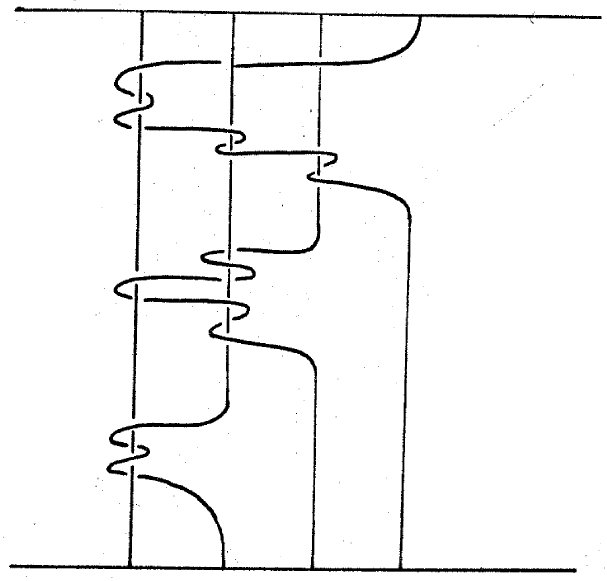
\includegraphics[scale=0.4]{Imagenes/peinado}
\end{turn}
\caption{Trenza peinada.}\label{peinada}
\end{figure}
%PEDIR DIBUJOS A JUAN


\section{Solución al problema de la palabra}\label{simples}

Supongamos que tenemos que decidir si una palabra $\beta\in B_n$ representa el elemento neutro. En primer lugar, mediante el homomorfismo $\eta$ de \ref{extension} comprobamos si la permutación que induce $\beta$ es la identidad. En caso de no serlo, sabemos que $\beta$ no es trivial. Si $\eta(\beta)=Id\in\Sigma_n$, entonces $\beta$ es pura por definición, por lo que trataremos de expresarla como elemento del producto semidirecto de grupos libres, ya que será trivial si y solo si cada uno de los factores lo es. Sin embargo, para conseguir esta expresión tenemos que escribir $\beta$ como producto de los generadores de Birman, puesto que estos son los que representan cada grupo libre.

Para ello, hagamos la siguiente consideración: dada una permutación $\tau\in\Sigma_n$ podemos encontrar una trenza que induzca esta permutación. Además podemos hacerlo de forma inyectiva, pues para permutaciones distintas daremos trenzas distintas. Esto da lugar a una \emph{sección conjuntista} (no es homomorfismo de grupos) en \ref{extension} $\varphi:\Sigma_n\to B_n$. Estas trenzas pueden ser elegidas de modo que todos los cruces sean positivos y cada par de cuerdas solo se cruce una vez. Para ello, empezamos por el $n$-ésimo punto y vamos asignando los demás de modo que las cuerdas siempre pasen por debajo de las ya existentes a las que tengan que cruzar y evitamos repetir de forma consecutiva algún $\sigma_i$. A estas trenzas las llamaremos \emph{trenzas simples} o \emph{trenzas de permutación}. Como toda permutación se puede expresar como producto de transposiciones, las trenzas simples tendrán la forma $\sigma_{i_1}\cdots\sigma_{i_l}$ para algún $1\leq l\leq n$, de modo que $\sigma_{i_j}\neq\sigma_{i_{j+1}}$ en cualquier palabra que represente a la trenza.  


Vamos a explicar en qué consiste entonces el algoritmo para resolver el problema de la palabra. Supongamos que tenemos una trenza $\sigma_{i_1}^{\pm 1}\sigma_{i_2}^{\pm 1}\cdots\sigma_{i_l}^{\pm 1}$. Vamos a multiplicar a izquierda y derecha cada generador por unas ciertas trenzas de permutación y sus inversas, de modo que nos quede un producto de trenzas puras que, por la forma que tendrá, será más sencillo de expresar en función de los generadores de Birman. Podemos empezar considerando la permutación $s_0=Id$, de modo que $\varphi(s_0)=1$. A continuación, tenemos que anular la permutación de $\sigma_{i_1}$, por lo que elegimos $s_1$ tal que $\varphi(s_1)=\sigma_{i_1}$ y hacemos el producto
\[
(\varphi(s_0)\sigma_{i_1}^{\pm 1}\varphi(s_1)^{-1})\varphi(s_1)\sigma_{i_2}^{\pm 1}\cdots\sigma_{i_l}^{\pm 1}.
\]
En el siguiente paso tenemos que anular la permutación de $\varphi(s_1)\sigma_{i_2}^{\pm 1}$, así que elegimos $s_2$ tal que $\varphi(s_2)=\sigma_{i_2}$ y hacemos el producto
\[
(\varphi(s_0)\sigma_{i_1}^{\pm 1}\varphi(s_1)^{-1})(\varphi(s_1)\sigma_{i_2}^{\pm 1}\varphi(s_2)^{-1}\varphi(s_1)^{-1})\varphi(s_1)\varphi(s_2)\cdots\sigma_{i_l}^{\pm 1}.
\]

%Lo de usar trenzas simples es porque la idea era que en cada paso solo se vaya moviendo una cuerda alrededor de las otras

Así iríamos reiterando hasta llegar al final de la palabra. Obsérvese que al sustituir, muchos términos se cancelarán y otros quedarán con una cierta simetría que facilitará expresarlos como producto de los generadores de Birman. En cualquier caso, como hay $n!$ trenzas de permutación y $2(n-1)$ generadores contando las potencias negativas, hay a lo sumo $n!2(n-1)$ factores distintos para expresarlos como producto de los generadores de Birman. Al ser una cantidad finita, siempre es teóricamente factible hacer una lista para transformarlos automáticamente. Una vez que tengamos una palabra de la forma
\[
A_{i_1,j_1}^{\pm 1}\cdots A_{i_r,j_r}^{\pm 1},
\]

basta usar los dos conjuntos de relaciones del grupo de trenzas puras definidas en el primer capítulo para reordenarlos de modo que queden de la forma
\[
(A_{i_{1,n},n+1}^{\pm 1}\cdots A_{i_{l,n},n+1}^{\pm 1})\cdots(A_{i_{1,1},3}^{\pm 1}\cdots A_{i_{k,1},3}^{\pm 1}) A_{12}^{\pm p}
\]
o equivalentemente en orden contrario (posiblemente algunos de los generadores no aparezcan). Una vez expresada así, ya basta comprobar si alguno de los factores no es trivial, que como cada uno está en un grupo libre sabemos que se puede resolver.


\begin{ej}
Sea $\beta=\sigma_1\sigma_2^{-1}\sigma_2^{-1}\sigma_3^{-1}\sigma_3^{-1}\sigma_1\in B_4$. Vamos a decidir si $\beta$ es trivial. En primer lugar calculamos su permutación inducida, $(12)(23)(23)(34)(34)(12)=Id$, por lo que la trenza es pura. Así que vamos utilizar las trenzas simples para expresarla como producto de los generadores de Birman. 
\begin{gather*}
(1\sigma_1\underline{\sigma_1^{-1}})(\underline{\sigma_1}\sigma_2^{-1}\underline{\sigma_2^{-1}\sigma_1^{-1}})(\underline{\sigma_1\sigma_2}\sigma_2^{-1}\underline{\sigma_1^{-1}})(\underline{\sigma_1}\sigma_3^{-1}\underline{\sigma_3^{-1}\sigma_1^{-1}})(\underline{\sigma_1\sigma_3}\sigma_3^{-1}\underline{\sigma_1^{-1}})(\underline{\sigma_1}\sigma_1 1)=\\
(\sigma_1\sigma_2^{-1}\sigma_2^{-1}\sigma_1^{-1})(\sigma_1\sigma_1^{-1}\sigma_3^{-1}\sigma_3^{-1})A_{12}=\\
(\sigma_1\sigma_2^{-1}\sigma_2^{-1}\sigma_1^{-1})A_{34}^{-1}A_{12}.
\end{gather*}

Nos quedan entonces un factor que expresar como producto de los generadores de Birman. Tenemos que
 
\begin{align*}
\sigma_1\sigma_2^{-1}\sigma_2^{-1}\sigma_1^{-1}=& \sigma_2^{-1}\underline{\sigma_2\sigma_1\sigma_2}\sigma_2^{-1}\sigma_2^{-1}\sigma_2^{-1}\sigma_1^{-1}=(\sigma_2^{-1})\sigma_1\sigma_2\sigma_1\sigma_2^{-1}\sigma_2^{-1}\sigma_2^{-1}\sigma_1^{-1}\\
&=(\sigma_2^{-1})\sigma_1\sigma_2\sigma_1\sigma_2^{-1}\sigma_2^{-1}\underline{\sigma_2^{-1}\sigma_1^{-1}\sigma_2^{-1}}(\sigma_2)=(\sigma_2^{-1})\sigma_1\sigma_2\sigma_1\sigma_2^{-1}\underline{\sigma_2^{-1}\sigma_1^{-1}\sigma_2^{-1}}(\sigma_1^{-1}\sigma_2)\\
&=(\sigma_2^{-1})\sigma_1\sigma_2\sigma_1\underline{\sigma_2^{-1}\sigma_1^{-1}\sigma_2^{-1}}(\sigma_1^{-1}\sigma_1^{-1}\sigma_2)=(\sigma_2^{-1})\sigma_1\sigma_2\sigma_1\sigma_1^{-1}\sigma_2^{-1}\sigma_1^{-1}(\sigma_1^{-1}\sigma_1^{-1}\sigma_2)\\
&=(\sigma_2^{-1})(\sigma_1^{-1}\sigma_1^{-1}\sigma_2)= (\sigma_2^{-2})(\sigma_2\sigma_1^{-2}\sigma_2^{-1})(\sigma_2^2)\\
&=A_{23}^{-1}A_{13}^{-1}A_{23}
\end{align*}
Este hecho se puede observar geométricamente en la Figura \ref{peinado}.



Por tanto, $\beta=A_{23}^{-1}A_{13}^{-1}A_{23}A_{34}^{-1}A_{12}$. Todavía no la tenemos de la forma buscada pues el orden no es el correcto. Por tanto, usamos las relaciones del grupo de trenzas puras para expresarla en el orden correcto. De todos modos, en este caso ya sabemos que no será trivial porque aparece $A_{12}$, generador de $F_1$, pero continuaremos el algoritmo por mostrar un ejemplo completo.

En este caso moveremos $A_{12}$ hacia la izquierda con los siguientes pasos.

%Para ahorrar espacio usaremos la notación $a^b=b^{-1}ab$. Obsérvese que $(a^b)^c=a^{bc}$, pues $(a^b)^c=(b^{-1}ab)^c=c^{-1}b^{-1}abc=a^{bc}$. Así pues,
%\begin{gather*}
%A_{23}^{-1}A_{13}^{-1}\underline{A_{23}A_{34}^{-1}}A_{12}=\\
%A_{23}^{-1}A_{13}^{-1}\underline{( A_{34}^{-1}A_{24}^{-1}A_{34}^{-1}A_{24}A_{34}) A_{23}}A_{12}=
%\end{gather*}

\begin{gather*}
A_{23}^{-1}A_{13}^{-1}A_{23}\underline{A_{34}^{-1}A_{12}}=\\
A_{23}^{-1}A_{13}^{-1}\underline{A_{23}A_{12}}A_{34}^{-1}=\\
A_{23}^{-1}A_{13}^{-1}\underline{A_{12}(A_{13}A_{23}A_{13}^{-1})}A_{34}^{-1}=\\
A_{23}^{-1}\underline{A_{12}(A_{13}A_{23}A_{13}^{-1}A_{23}^{-1}A_{13}^{-1}}A_{13}A_{23}A_{13}^{-1})A_{34}^{-1}=\\
\underline{A_{12}(A_{13}A_{23}^{-1}A_{13}^{-1}}A_{13}A_{23}A_{13}^{-1}A_{23}^{-1}A_{13}^{-1}A_{13}A_{23}A_{13}^{-1})A_{34}^{-1}.
\end{gather*}
Tal como adelantábamos, claramente no es trivial.

\begin{figure}[h!]
\centering
\tikzset{decorate sep/.style 2 args=
{decorate,decoration={shape backgrounds,shape=circle,shape size=#1,shape sep=#2}}}
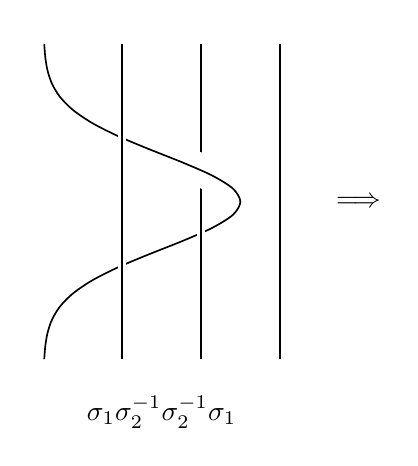
\begin{tikzpicture}
\draw[white,double=black,very thick,-] (-2,0) -- (-2,2);

\foreach \x in {-1}{
\draw[white,double=black,very thick,-] (\x,-2) -- (\x,2);
}
\draw[smooth,white,double=black,line width=2mm,-] plot[variable=\x,domain=-2:2] ({2.5*exp(-1.4*\x*\x)-4},{\x});
\draw[white,double=black,very thick,-] (-3,2) -- (-3,-2);
\draw[white,double=black,very thick,-] (-2,-2) -- (-2,0);
\node[anchor=south] at (-2.5,-3) {$\sigma_1\sigma_2^{-1}\sigma_2^{-1}\sigma_1$};
\node[anchor=south] at (0,-0.2) {$\Longrightarrow$};
\end{tikzpicture}\quad
\begin{tikzpicture}
\draw[white,double=black,very thick,-] (-4,-2) -- (-4,0);
\foreach \x in {-1}{
\draw[white,double=black,very thick,-] (\x,-2) -- (\x,2);
}
\draw[smooth,white,double=black,line width=2mm,-] plot[variable=\x,domain=-2:2] ({-2.5*exp(-1.4*\x*\x)-2},{\x});

\draw[white,double=black,very thick,-] (-3,-2) -- (-3,2);
\draw[white,double=black,very thick,-] (-4,2) -- (-4,0);
\node[anchor=south] at (-2.5,-3) {$\sigma_2^{-1}\sigma_1^{-1}\sigma_1^{-1}\sigma_2$};
\node[anchor=south] at (0,-0.2) {$\Longrightarrow$};
\end{tikzpicture}\quad
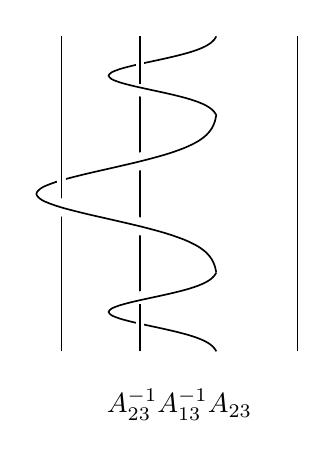
\begin{tikzpicture}
\draw[white,double=black,very thick,-] (-3,-1.3) -- (-3,1.3);
\draw[white,double=black,very thick,-] (-3,-1.4) -- (-3,1.3);
\draw[white,double=black,very thick,-] (-4,-2) -- (-4,0);
\foreach \x in {-1}{
\draw[white,double=black,very thick,-] (\x,-2) -- (\x,2);
}

\draw[smooth,white,double=black,line width=1mm,-] plot[variable=\x,domain=1:2] ({-1.4*exp(-15*(\x-1.5)*(\x-1.5))-2},{\x});
\draw[smooth,white,double=black,line width=1mm,-] plot[variable=\x,domain=-1:1] ({-2.3*exp(-5*(\x)*(\x))-2.018},{\x});
\draw[smooth,white,double=black,line width=1mm,-] plot[variable=\x,domain=-2:-1] ({-1.4*exp(-15*(\x+1.5)*(\x+1.5))-2},{\x});

\draw[white,double=black,very thick,-] (-4,2) -- (-4,0);
\draw[white,double=black,very thick,-] (-3,-2) -- (-3,-1.4);
\draw[white,double=black,very thick,-] (-3,1.4) -- (-3,2);

\node[anchor=south] at (-2.5,-3) {$A_{23}^{-1}A_{13}^{-1}A_{23}$};
\end{tikzpicture}
\caption{En el primer paso tiramos hacia la izquierda de la tercera cuerda, arrastrando con ella la primera, y en el segundo la vamos doblando.}\label{peinado}
\end{figure}

\end{ej}

Como hemos podido comprobar en el ejemplo anterior, la palabra se va haciendo exponencialmente más larga durante el proceso, convirtiendo este algoritmo en altamente ineficiente, hasta el punto de que el propio Artin comentara \cite{Artin}:

\emph{``Although it has been proved that every braid can be deformed into a similar normal form, the writer is
convinced that any attempt to carry this out on a living person would only lead to violent protests and
discrimination against mathematics. He would therefore discourage such an experiment''\footnote{``Aunque ha sido probado que toda trenza puede ser deformada en una forma normal similar, el escritor está convencido de que cualquier intento de llevar esto acabo por una persona viva solo llevaría a violentas protestas y discriminación hacia las matemáticas. Por tanto, desaconsejaría tal experimento''.}.}

Sin embargo, versiones mejoradas hasta tiempo polinomial pueden ser encontradas en \cite{polynomial}.



%\begin{figure}[!tbp]
%  \centering
%  \subfloat[Flower one.]{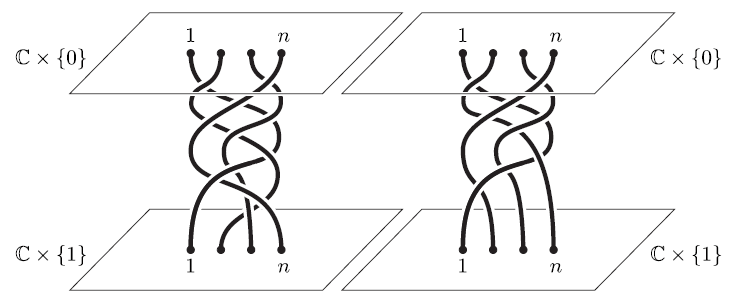
\includegraphics[width=0.5\textwidth]{Imagenes/hilos}\label{fig:f1}}
%  \hfill
%  \subfloat[Flower two.]{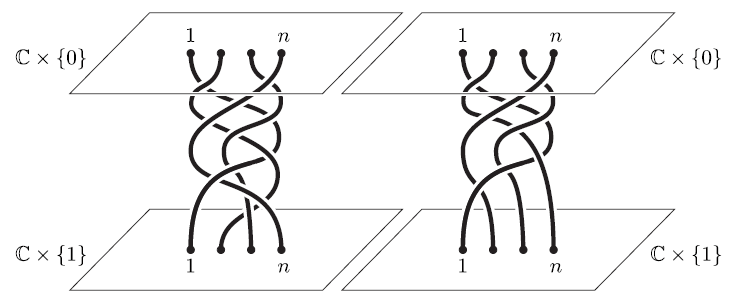
\includegraphics[width=0.5\textwidth]{Imagenes/hilos}\label{fig:f2}}
%  \caption{My flowers.}
%\end{figure}https://tex.stackexchange.com/questions/148438/putting-two-images-beside-each-other

%https://tex.stackexchange.com/questions/213075/two-tikzpictures-side-by-side



\end{document}